\section{Aufbau}
\begin{frame}
\frametitle{Grundaufbau}
	\begin{center}
		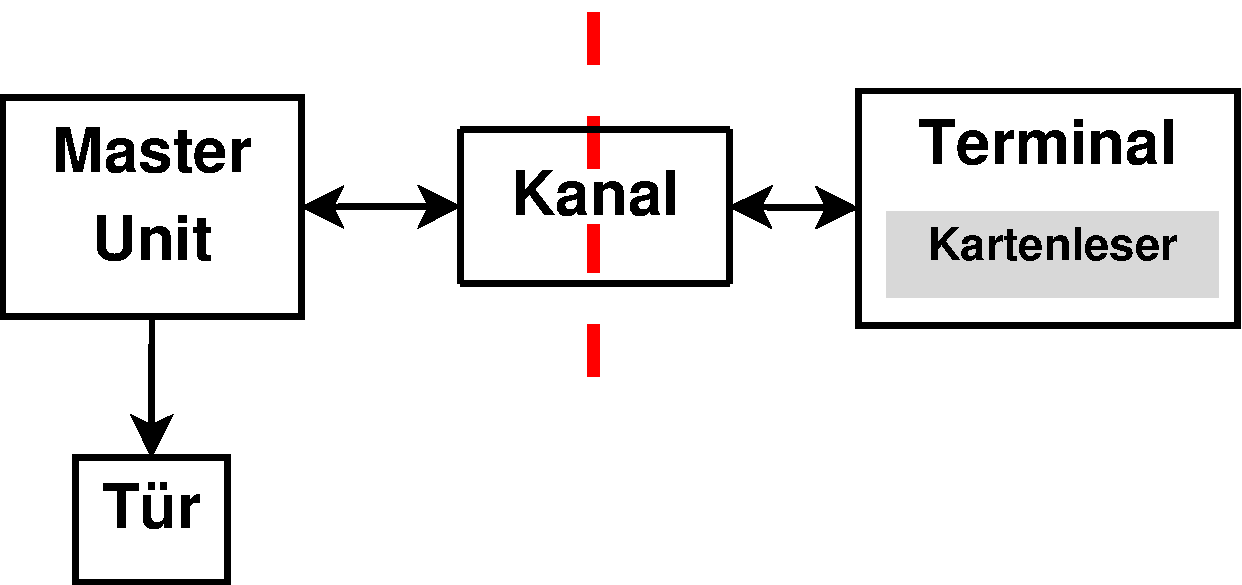
\includegraphics[width=210px]{grundaufbau}
	\end{center}
\end{frame}

\begin{frame}
\frametitle{Master Unit}
	\begin{itemize}
		\item<2-> Speicherung der Datenbank
		\item<3-> Authentifizierung der Nutzer
		\item<4-> L"oschung der Schl"ussel \& Datenbank bei physikalischen Angriffen
		\item<5-> USV
	\end{itemize}
\end{frame}

\begin{frame}
\frametitle{Panel}
	\begin{itemize}
		\item<2-> Weitergabe der Kartendaten
		\item<3-> Ein- und Ausgabe \small{(Master Unit <-> Mensch)}
		\item<4-> L"oschung des Schl"ussels bei physikalischen Angriffen
	\end{itemize}
\end{frame}

\begin{frame}
\frametitle{Kanal}
	Galvanische Trennung zwischen Master Unit und Panel
\end{frame}
